% UQ Gemini theme
% See: https://github.com/alfurka/gemini-uq
% Forked from
% https://rev.cs.uchicago.edu/k4rtik/gemini-uccs
% which is forked from
% https://github.com/anishathalye/gemini


\documentclass[final,20pt]{beamer}

% ====================
% Packages
% ====================
\usepackage[T1]{fontenc}
\usepackage{lmodern}
\usepackage[size=custom,width=121.9,height=91.425,scale=1.52375]{beamerposter}
\usetheme{gemini}
\usecolortheme{uchicago}
\usepackage{colortbl}
\usepackage{graphicx}
\usepackage{booktabs}
\usepackage{tikz}
\usepackage{tabularx}  % for flexible column widths
\usepackage{multirow}   % for multirow cells
\usepackage{pgfplots}
\pgfplotsset{compat=1.17}
\usepackage{soul}
% or any other color you prefer

% ====================
% Lengths
% ====================

% If you have N columns, choose \sepwidth and \colwidth such that
% (N+1)*\sepwidth + N*\colwidth = \paperwidth
\newlength{\sepwidth}
\newlength{\colwidth}
\setlength{\sepwidth}{0.025\paperwidth}
\setlength{\colwidth}{0.3\paperwidth}

\newcommand{\separatorcolumn}{\begin{column}{\sepwidth}\end{column}}


% ====================
% Title
% ====================

\title{Optimizing Keyboard Layouts for English Text}
\author{\textbf{David Sommerfield -- Computer Science Department} } % \inst{1} \and Advisor \inst{2}

% ====================
% Footer (optional)
% ====================


% ====================
% Footer (optional)
% ====================

\footercontent{}

% (can be left out to remove footer)

% ====================
% Logo (optional)
% ====================

% use this to include logos on the left and/or right side of the header:
% \logoright{\includegraphics[height=7cm]{logo1.pdf}}
% \logoleft{\includegraphics[height=7cm]{logo2.pdf}}

% ====================
% Body
% ====================



\begin{document}
\addtobeamertemplate{headline}{}
{
    \begin{tikzpicture}[remember picture,overlay]
      \node [anchor=north west, inner sep=3cm] at ([xshift=0.0cm,yshift=3.6666cm]current page.north west)
      {
\includegraphics[height=9.752cm]{logos/winona.eps}};
      
      \node [anchor=north east, inner sep=3cm] at ([xshift=0.0cm,yshift=2.777cm]current page.north east)
      {
\includegraphics[height=9.752cm]{logos/qr-code.pdf}};
    \end{tikzpicture}
}

\begin{frame}[t]
\begin{columns}[t]
\separatorcolumn

\begin{column}{\colwidth}
  \begin{alertblock}{Introduction}
Layout optimization is difficult and historically has relied on theoretical decisions or manual observations of data instead of statistically robust modeling. QWERTY, a product of these observations, was popularized by its usage on typewriters in the 1870s and, in spite of its age, remains as the most common keyboard layout today. The search space for layouts grows factorially, making it impossible to search exhaustively, necessitating smart ways of searching, such as metaheuristic optimization techniques like simulated annealing and genetic algorithms. The focus of this project is implementing such a technique on a predictive model of typing speed (R$^2$:$0.78$, MAE:$12.7$ms) to generate a layout optimized with real-world data, remedying the shortcomings of traditional layout optimization methods.



  \end{alertblock}

\begin{block}{Data Processing}
      Two data sets are used to construct a predictive model of typing time: The 136M Keystrokes Dataset for data on keystroking patterns and their correlation with typing speed and the iWeb corpus for ngram frequency information.

      \heading{The 136M Keystrokes Dataset} % The inclusion of these layouts helps prevent overfitting.
    This dataset comprises 8,228 hours of typing data from 168,000 volunteers across four keyboard layouts: azerty, dvorak, qwerty, and qwertz. Data is limited to participants who used 9 to 10 fingers for typing to approximate touch typing and ensure consistency in the input methodology. Approximate string matching is used to identify typos; then, a sliding window is used to decompose the data into bistrokes and tristrokes. Transition times for each typo-free nstroke are grouped by key-coordinate ngram pairs and then averaged with outliers being removed by IQR.


    \begin{figure}[h]
    \begin{center}
    \small
    \renewcommand{\arraystretch}{1.5}
    \begin{tabularx}{\textwidth}{ | *{10}{>{\centering\arraybackslash}X|} }
    \hline    
\cellcolor[HTML]{24314b}\textbf{M} & \cellcolor[HTML]{316799}\textbf{R} & \cellcolor[HTML]{3091ca}\textbf{T} & \cellcolor[HTML]{283a59}\textbf{C} & \cellcolor[HTML]{20293f}\textbf{W} & \cellcolor[HTML]{1b2131}\textbf{,} & \cellcolor[HTML]{181e2c}\textbf{K} & \cellcolor[HTML]{3183ba}\textbf{A} & \cellcolor[HTML]{1DC8FF}\textbf{E} & \cellcolor[HTML]{131722}\textbf{'} \\ \hline
\cellcolor[HTML]{2d4a71}\textbf{L} & \cellcolor[HTML]{3173a8}\textbf{N} & \cellcolor[HTML]{2b4366}\textbf{D} & \cellcolor[HTML]{316a9d}\textbf{S} & \cellcolor[HTML]{1b2132}\textbf{V} & \cellcolor[HTML]{222c43}\textbf{Y} & \cellcolor[HTML]{283958}\textbf{U} & \cellcolor[HTML]{3180b7}\textbf{O} & \cellcolor[HTML]{3173a9}\textbf{I} & \cellcolor[HTML]{222e45}\textbf{G} \\ \hline
\cellcolor[HTML]{2e507a}\textbf{H} & \cellcolor[HTML]{131621}\textbf{X} & \cellcolor[HTML]{12141e}\textbf{Z} & \cellcolor[HTML]{1e2538}\textbf{B} & \cellcolor[HTML]{232e46}\textbf{F} & \cellcolor[HTML]{1b2233}\textbf{.} & \cellcolor[HTML]{131722}\textbf{-} & \cellcolor[HTML]{12141e}\textbf{Q} & \cellcolor[HTML]{12151f}\textbf{J} & \cellcolor[HTML]{222d45}\textbf{P} \\ \hline
\multicolumn{10}{|c|}{\multirow{1}{*}{\textbf{SPACE}}} \\ \hline
    \end{tabularx}
    \end{center}
    
    
    \begin{center}
    \small
    \renewcommand{\arraystretch}{1.5}
    \begin{tabularx}{\textwidth}{ | *{10}{>{\centering\arraybackslash}X|} }
    \hline
    % $(-5,4)$ & $(-4,4)$ & $(-3,4)$ & $(-2,4)$ & $(-1,4)$ & $(1,4)$ & $(2,4)$ & $(3,4)$ & $(4,4)$ & $(5,4)$\\ \hline
    \textbf{$(-5,3)$} & \textbf{$(-4,3)$} & \textbf{$(-3,3)$} & \textbf{$(-2,3)$} & \textbf{$(-1,3)$} & \textbf{$(1,3)$} & \textbf{$(2,3)$} & \textbf{$(3,3)$} & \textbf{$(4,3)$} & \textbf{$(5,3)$}\\ \hline
    \textbf{$(-5,2)$} & \textbf{$(-4,2)$} & \textbf{$(-3,2)$} & \textbf{$(-2,2)$} & \textbf{$(-1,2)$} & \textbf{$(1,2)$} & \textbf{$(2,2)$} & \textbf{$(3,2)$} & \textbf{$(4,2)$} & \textbf{$(5,2)$}\\ \hline
    \textbf{$(-5,1)$} & \textbf{$(-4,1)$} & \textbf{$(-3,1)$} & \textbf{$(-2,1)$} & \textbf{$(-1,1)$} & \textbf{$(1,1)$} & \textbf{$(2,1)$} & \textbf{$(3,1)$} & \textbf{$(4,1)$} & \textbf{$(5,1)$} \\ \hline
\multicolumn{10}{|c|}{\multirow{1}{*}{\textbf{$(0,0)$}}} \\ \hline
    \end{tabularx}
    \end{center}
    \caption{Key-coordinate Character Mapping and Frequency Heatmap}
    \label{fig:keyboard1}
    \end{figure}

    % The processed data was decomposed into ngrams and nstrokes, with a proposed model correlating ngram frequency and typing speed, considering featural positions for accurate prediction.

  \end{block}

\end{column}

\separatorcolumn
\begin{column}{\colwidth}
    \begin{figure}[h]
    \begin{center}
    \begin{tabular}{l|l}
    \textbf{Typing Error} & \textbf{Example String} \\ \hline
    % None & But thank you for the offer \\
    Insertion      & But thank\textcolor{brillaintblue}{\underline{\textcolor{white}{k}}} you for the offer                     \\
    Deletion       & But tha\textcolor{brillaintblue}{\underline{\hspace{0.2em}}}k you for the offer                       \\
    Substitution   & But tha\textcolor{brillaintblue}{\underline{\textcolor{white}{b}}}k you for the offer                      \\
    \end{tabular}
    \end{center}
    \caption{Types of Typing Errors}
    \label{fig:typing_errors}
    \end{figure}

    
    \heading{iWeb Corpus}
    The iWeb corpus is a comprehensive collection of high-quality text and one of the largest available English corpora. A sliding window decomposes it into bigrams and trigrams, capturing their frequency of occurrence.

    \begin{figure}[h]
    \begin{table}[h]
    \begin{tabular}{lllll}
    \textbf{Bigram} & \textbf{Occurences} &  & \textbf{Trigram} & \textbf{Occurences} \\
    th              & 9709171             &  & the              & 6076523             \\
    he              & 8552661             &  & ing              & 3227179             \\
    in              & 7913861             &  & and              & 2998065             \\
    an              & 6389345             &  & ion              & 1716878             \\
    er              & 6348583             &  & ent              & 1519196            
    \end{tabular}
    \end{table}
    \caption{Top 5 Bigrams and Trigrams Extracted from the Corpus}
    \label{fig:ngrams}
    \end{figure}
    
  \begin{block}{Defining The Cost Function}
         \heading{Data Analysis}
         Ngram frequency significantly influences typing speed, with a high frequency aiding muscle memory regardless of placement. After accounting for the effect of frequency, we can assess the influence of key placement and identify three distinct categories of bistroke:

    \begin{itemize}
      \item \textbf{ALT:} Alternating bistroke. A bigram typed on both hands by alternating sides of the keyboard. Fastest category.
      \item \textbf{SHB:} same-hand bistroke. Opposite of an ALT.
      \item \textbf{SFB:} same-finger bistroke. A bigram typed using the same finger twice. Slowest category, especially for high WPMs.
    \end{itemize}

    \begin{figure}[h]
        \centering
        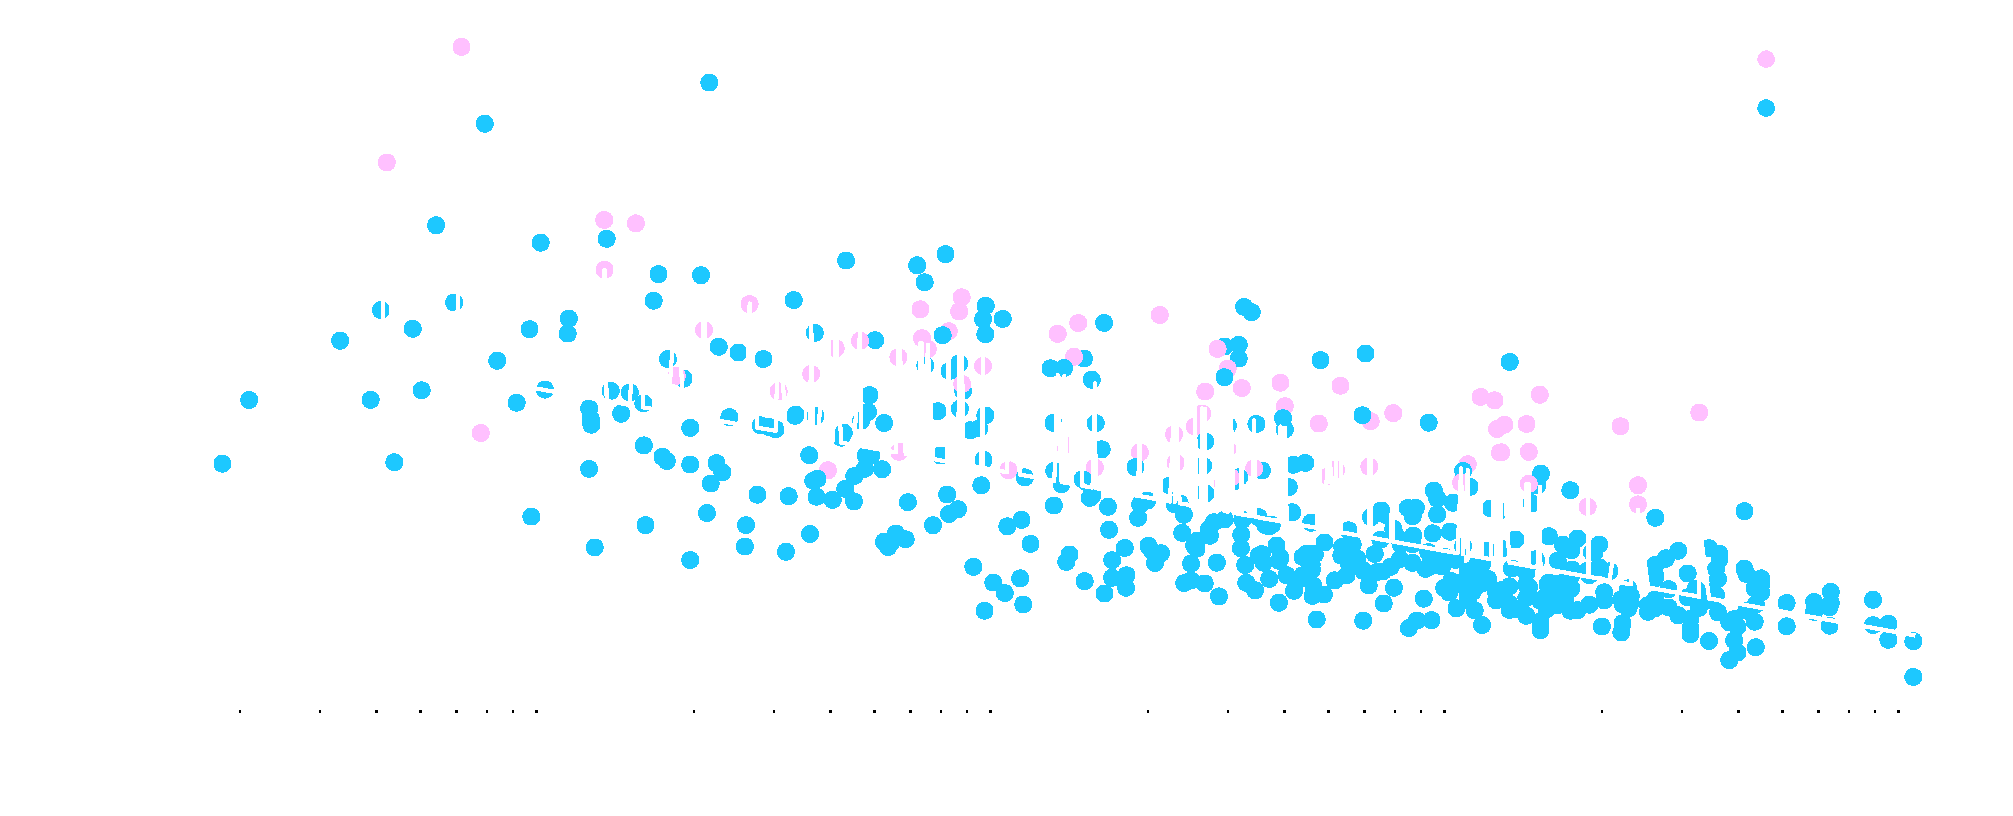
\includegraphics[width=\textwidth]{logos/plot.pdf}
        \caption{The Effect of SFBs and Frequency on Typing Speed (>80WPM)}
        \label{fig:sfbspeed}
    \end{figure}

  \end{block}
\end{column}

\separatorcolumn

\begin{column}{\colwidth}
    \heading{Cost Function Construction}
    To prevent overfitting on our sparse data, we devise a cost function from our findings. Using the Levenberg-Marquardt algorithm the parameters are fine-tuned to fit the typing data. For a bistroke $b$, of category $i = \{1,2,3\}$, the cost is: \justifying
    \begin{equation*}
        C(b)  = \left(p_0 \log (f(b) + p_1) + p_2\right) 
        \times
        \left(1 + P_x(b) P_y(b) +  P^{(i)}_x(b)  P^{(i)}_y(b) \Delta \right)  
    \end{equation*}
    $\Delta$ is the row-stagger adjusted distance between keys if it's an SFB and $1$ otherwise. $P_x$ and $P_x$ are row and column penalties. \justifying
  
    For a tristroke $t$, the cost is: 
    \begin{equation*}
    C(t) = C(b_1(t)) + C(b_2(t)) + P_x(s(t))  P_y(s(t)) \Delta
    \end{equation*}
    $b_1(t), b_2(t)$ are the constituent bistrokes of $t$, $S(t)$ is its associated skipstroke, and $\Delta$ represents the distance if a skipstroke is present, and $0$ otherwise. For fast typists, same-finger skipstrokes (strokes separated by one stroke sharing a finger) behave more like delayed same-finger bistrokes. The final cost of a layout $l$ is the sum of every tristroke's cost $\times$ frequency, effectively estimating the typing time for a given layout $C(l) = \sum_{t \in T} (C(t) \times f(t) )$
    \justifying

        
  \begin{block}{Simulated Annealing}
    Simulated annealing optimizes by gradually reducing the probability of accepting suboptimal moves over time. The acceptance probability is guided by the temperature parameter and a cooling schedule that diminishes it. For our problem space, a move is simply swapping two keys. The full algorithm is outlined below:

    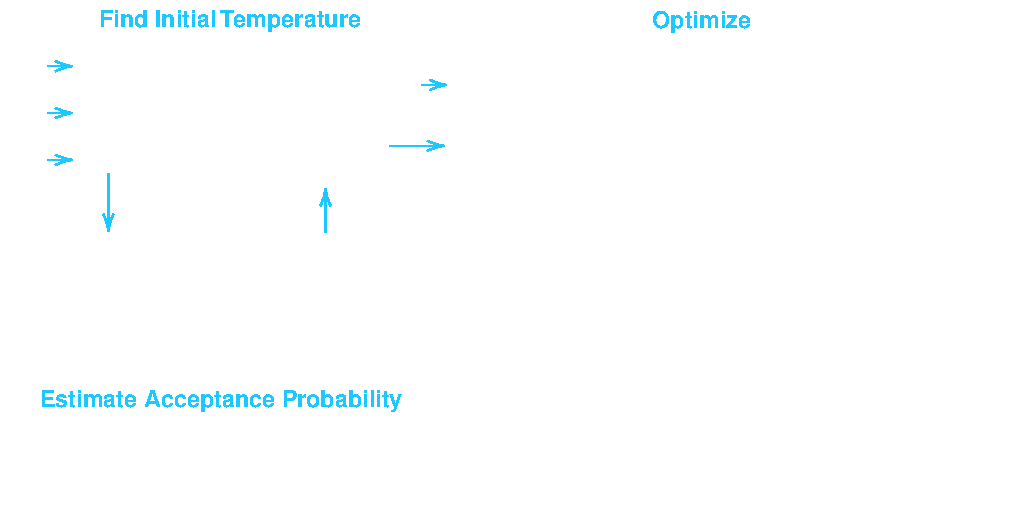
\includegraphics[width=\textwidth]{sa.pdf}

  \end{block}

  \begin{alertblock}{Results and Future Work}
    For the final result (fig. 1), a layout of the most common $30$ characters was optimized. According to the time prediction model, the converged solution is $8\%$ quicker than QWERTY. To create better predictive models in the future, we developed an open-source tool called Kiakl to collect more diverse keystroke data from volunteers on a greater variety of alternative layouts.
  \end{alertblock}


\end{column}

\separatorcolumn
\end{columns}
\end{frame}

\end{document}
